\documentclass[letterpaper,14pt,titlepage,fleqn]{article}

\setlength{\mathindent}{1cm}

\usepackage{graphicx}                                        

\usepackage{amssymb}                                         
\usepackage{amsmath}                                         
\usepackage{amsthm}                                          

\usepackage{alltt}                                           
\usepackage{float}
\usepackage{color}

\usepackage{url}

\usepackage{balance}
\usepackage[TABBOTCAP, tight]{subfigure}
\usepackage{enumitem}

\usepackage{pstricks, pst-node}

\usepackage{cite}
\usepackage{indentfirst}
\usepackage{listings}

% the following sets the geometry of the page
\usepackage{geometry}
\geometry{textheight=9in, textwidth=6.5in}

% random comment

\newcommand{\cred}[1]{{\color{red}#1}}
\newcommand{\cblue}[1]{{\color{blue}#1}}

\usepackage{hyperref}

\usepackage{textcomp}
\usepackage{listings}

\def\name{Haoxiang Wang; Student ID: 932359049}

%% The following metadata will show up in the PDF properties
\hypersetup{
  colorlinks = true,
  urlcolor = black,
  pdfauthor = {\name},
  pdfkeywords = {CS557 Project 5},
  pdftitle = {Project \#5: Image Manipulation in a "Magic Lens"},
  pdfsubject = {Project \#5: Image Manipulation in a "Magic Lens"},
  pdfpagemode = UseNone
}

\parindent = 0.0 in
\parskip = 0.2 in

\author{\name}
\title{Project \#5: Image Manipulation in a "Magic Lens"}

\begin{document}
\maketitle

This project is the fifth project I have done in this class, and it is the first project that using GLSL to implement image processing effects. Since I gained the experience of image processing from my research project, this project seems easy to deal with, and the result turned out that the project was also fun to play with. The whole project only takes me a few hours to get everything done and fit to all the requirements. The results images and the explanation of how code works will be described in the after section. 

\section{Source Listing}
In this project, three files are necessary. They are .glib file, .vert file, and .frag file. No .obj file is needed in this project. The specific filenames and usages are listed below.

mag.glib --- Handle the user interface and object

mag.vert --- Handle the vertex shader

mag.frag --- handle the fragment shader

\section{Result Images and Explanation}
The requirements of this project can be simply divided into three parts and one extra part. The whole project is trying to implement a ``magic lens'' which contains the magnification, rotation, and sharpening. The first one is to implement the magnification, the second part is to implement the rotation, and the third part is to implement sharpening. The extra part of this project is changing the rectangle lens to a circle lens, which requires some extra work in the code. The image we are trying to add some effects on is treated as a texture mapped onto an X-Y Quad. The following image shows that original image and the variable values when the image is rendered. 
\begin{center}
	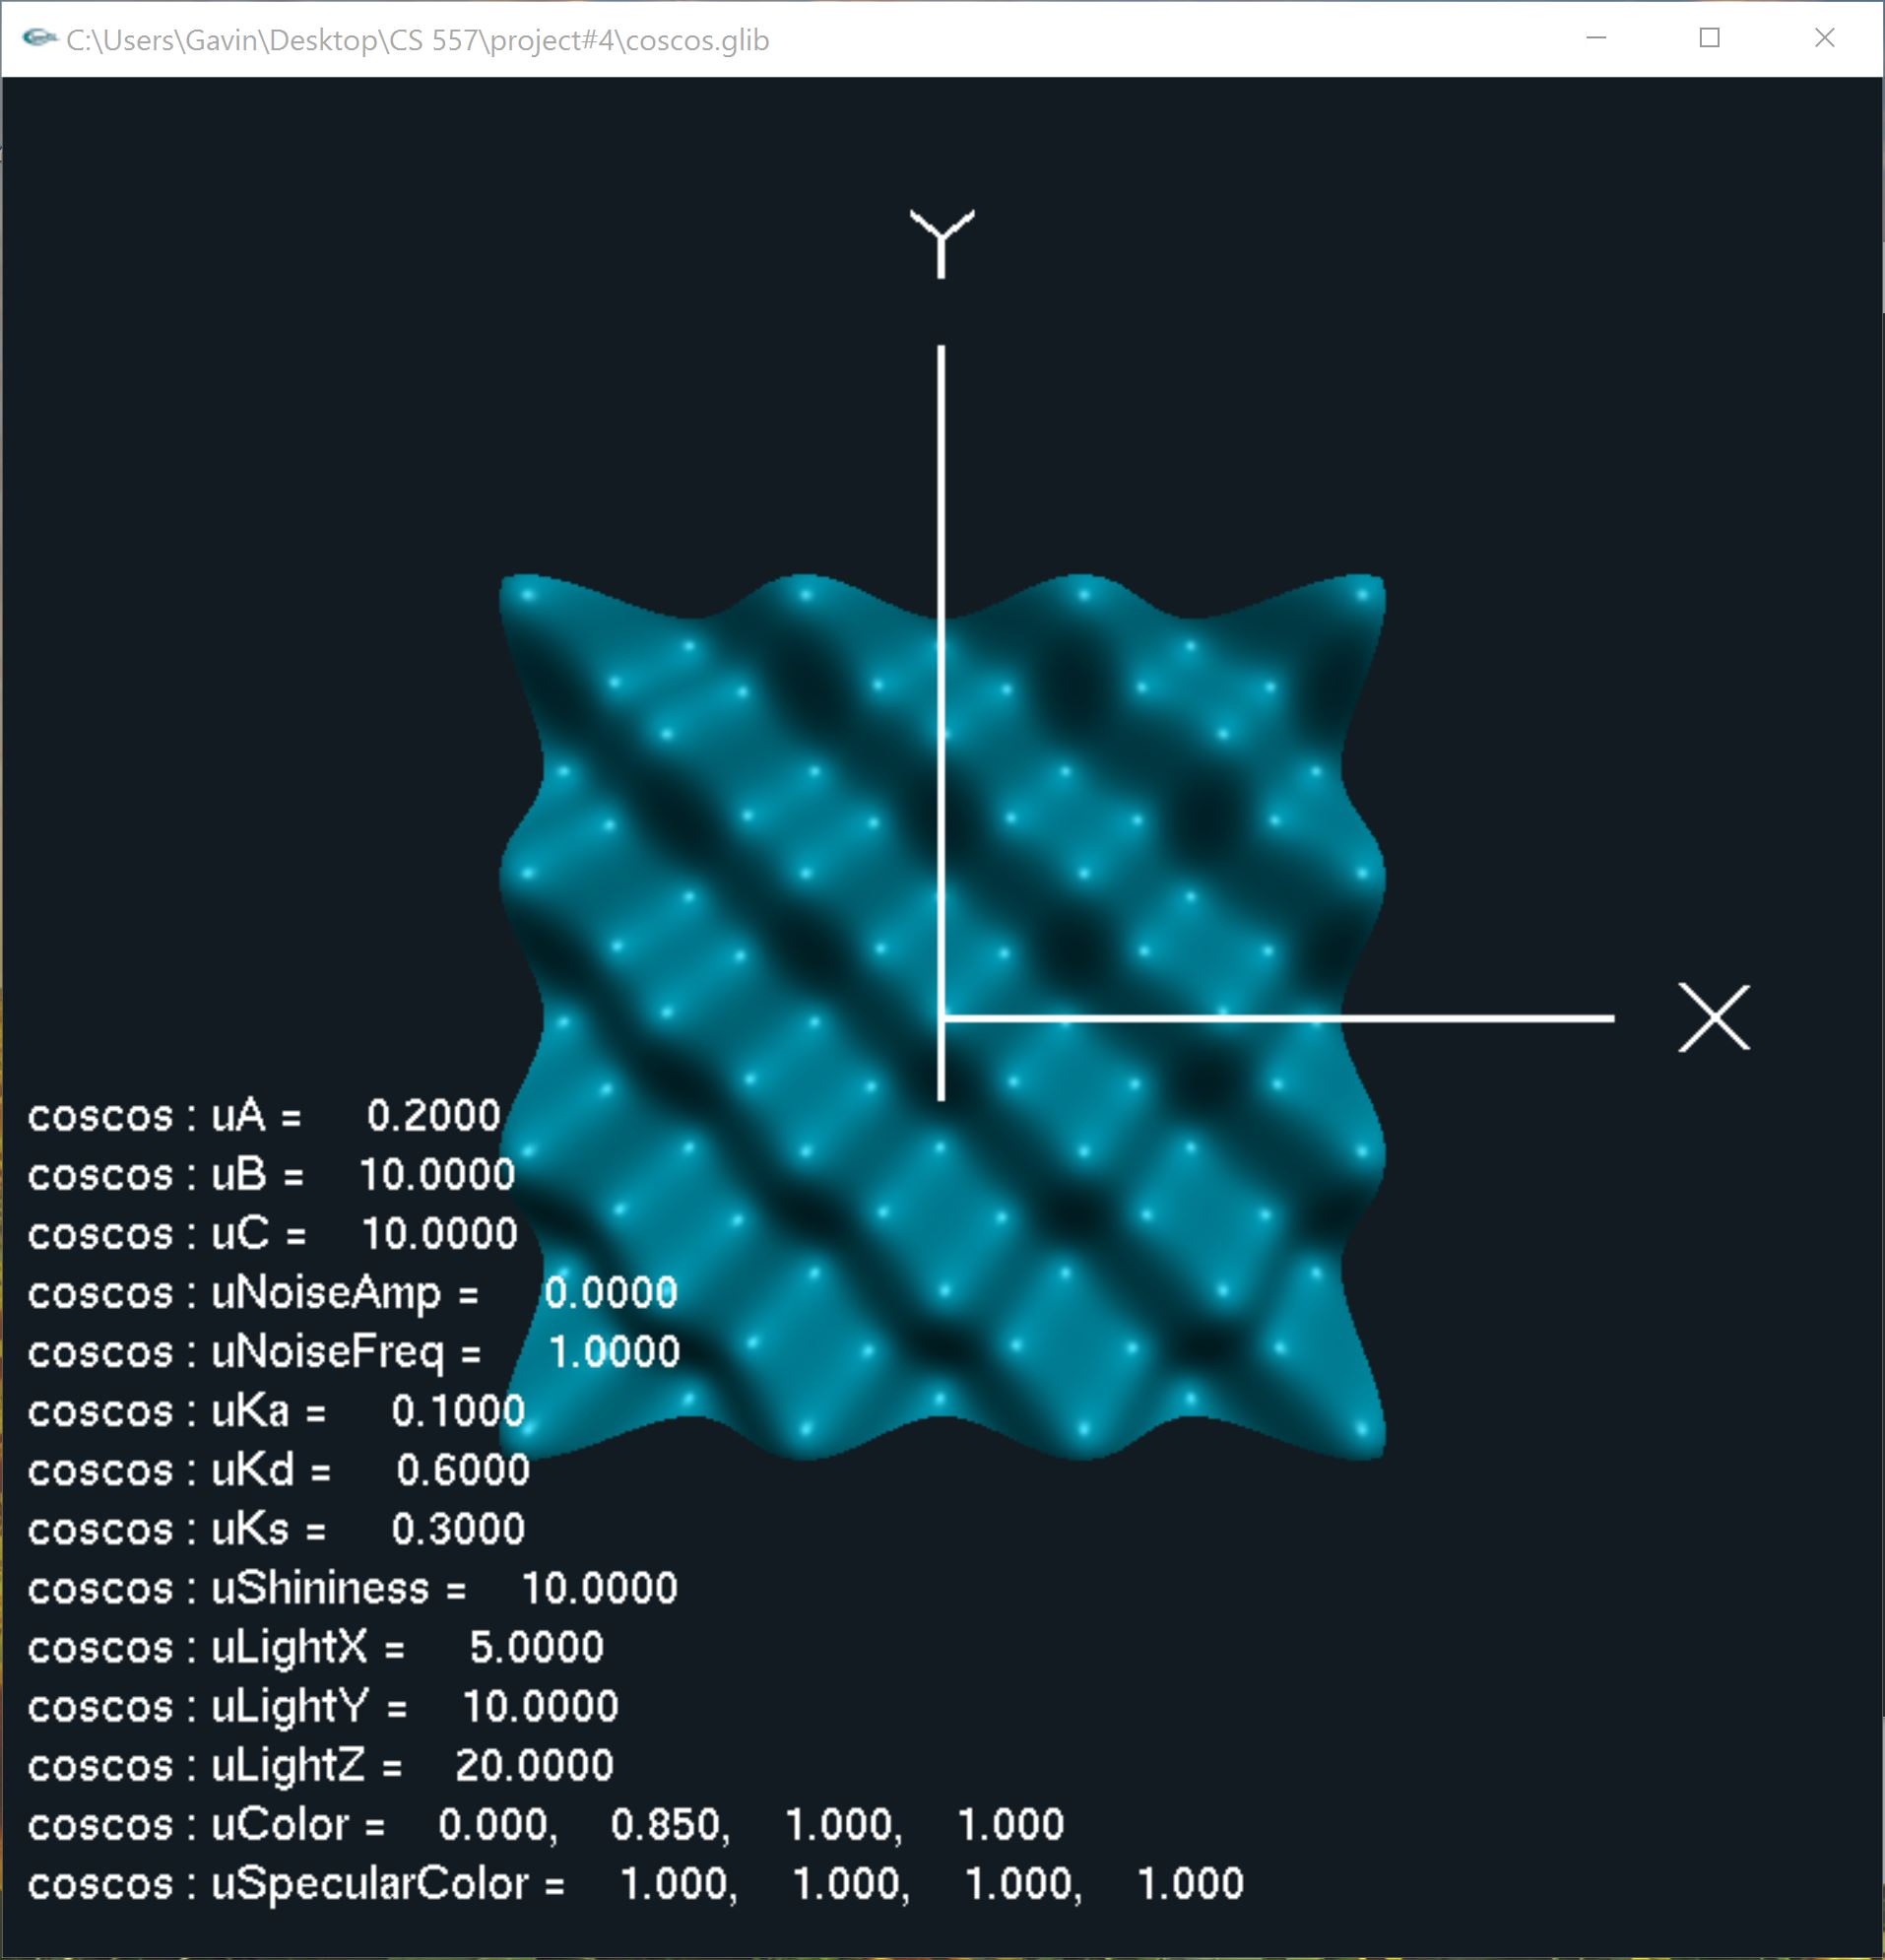
\includegraphics[width=3.2in]{origin.jpg}
\end{center}
The first part of the project is magnification. The part of the image covered by the lens will be ``enlarged'' by a coefficient getting from the slider named ``uMagFactor''. The effect is not the real magnification, it doesn't even contain the refraction implementation. the fact behind my magnification is playing with the st coordinates. By checking if the texel is in the $[uScenter-uDs/2 , uScenter+uDs/2]$ and $[uTcenter-uDt/2 , uTcenter+uDt/2]$ range, we could tell whether the texel should be manipulate or not. If the texel needs to be manipulated, I simply grab the rgb color from another texel and put it as itself's rgb value. The equations for searching the texels are $sp = (s - uScenter) / uMagFactor + uScenter$ and $tp = (t - uTcenter) / uMagFactor + uTcenter$. The following left image shows the effect of magnification on cat's eye.
\begin{center}
	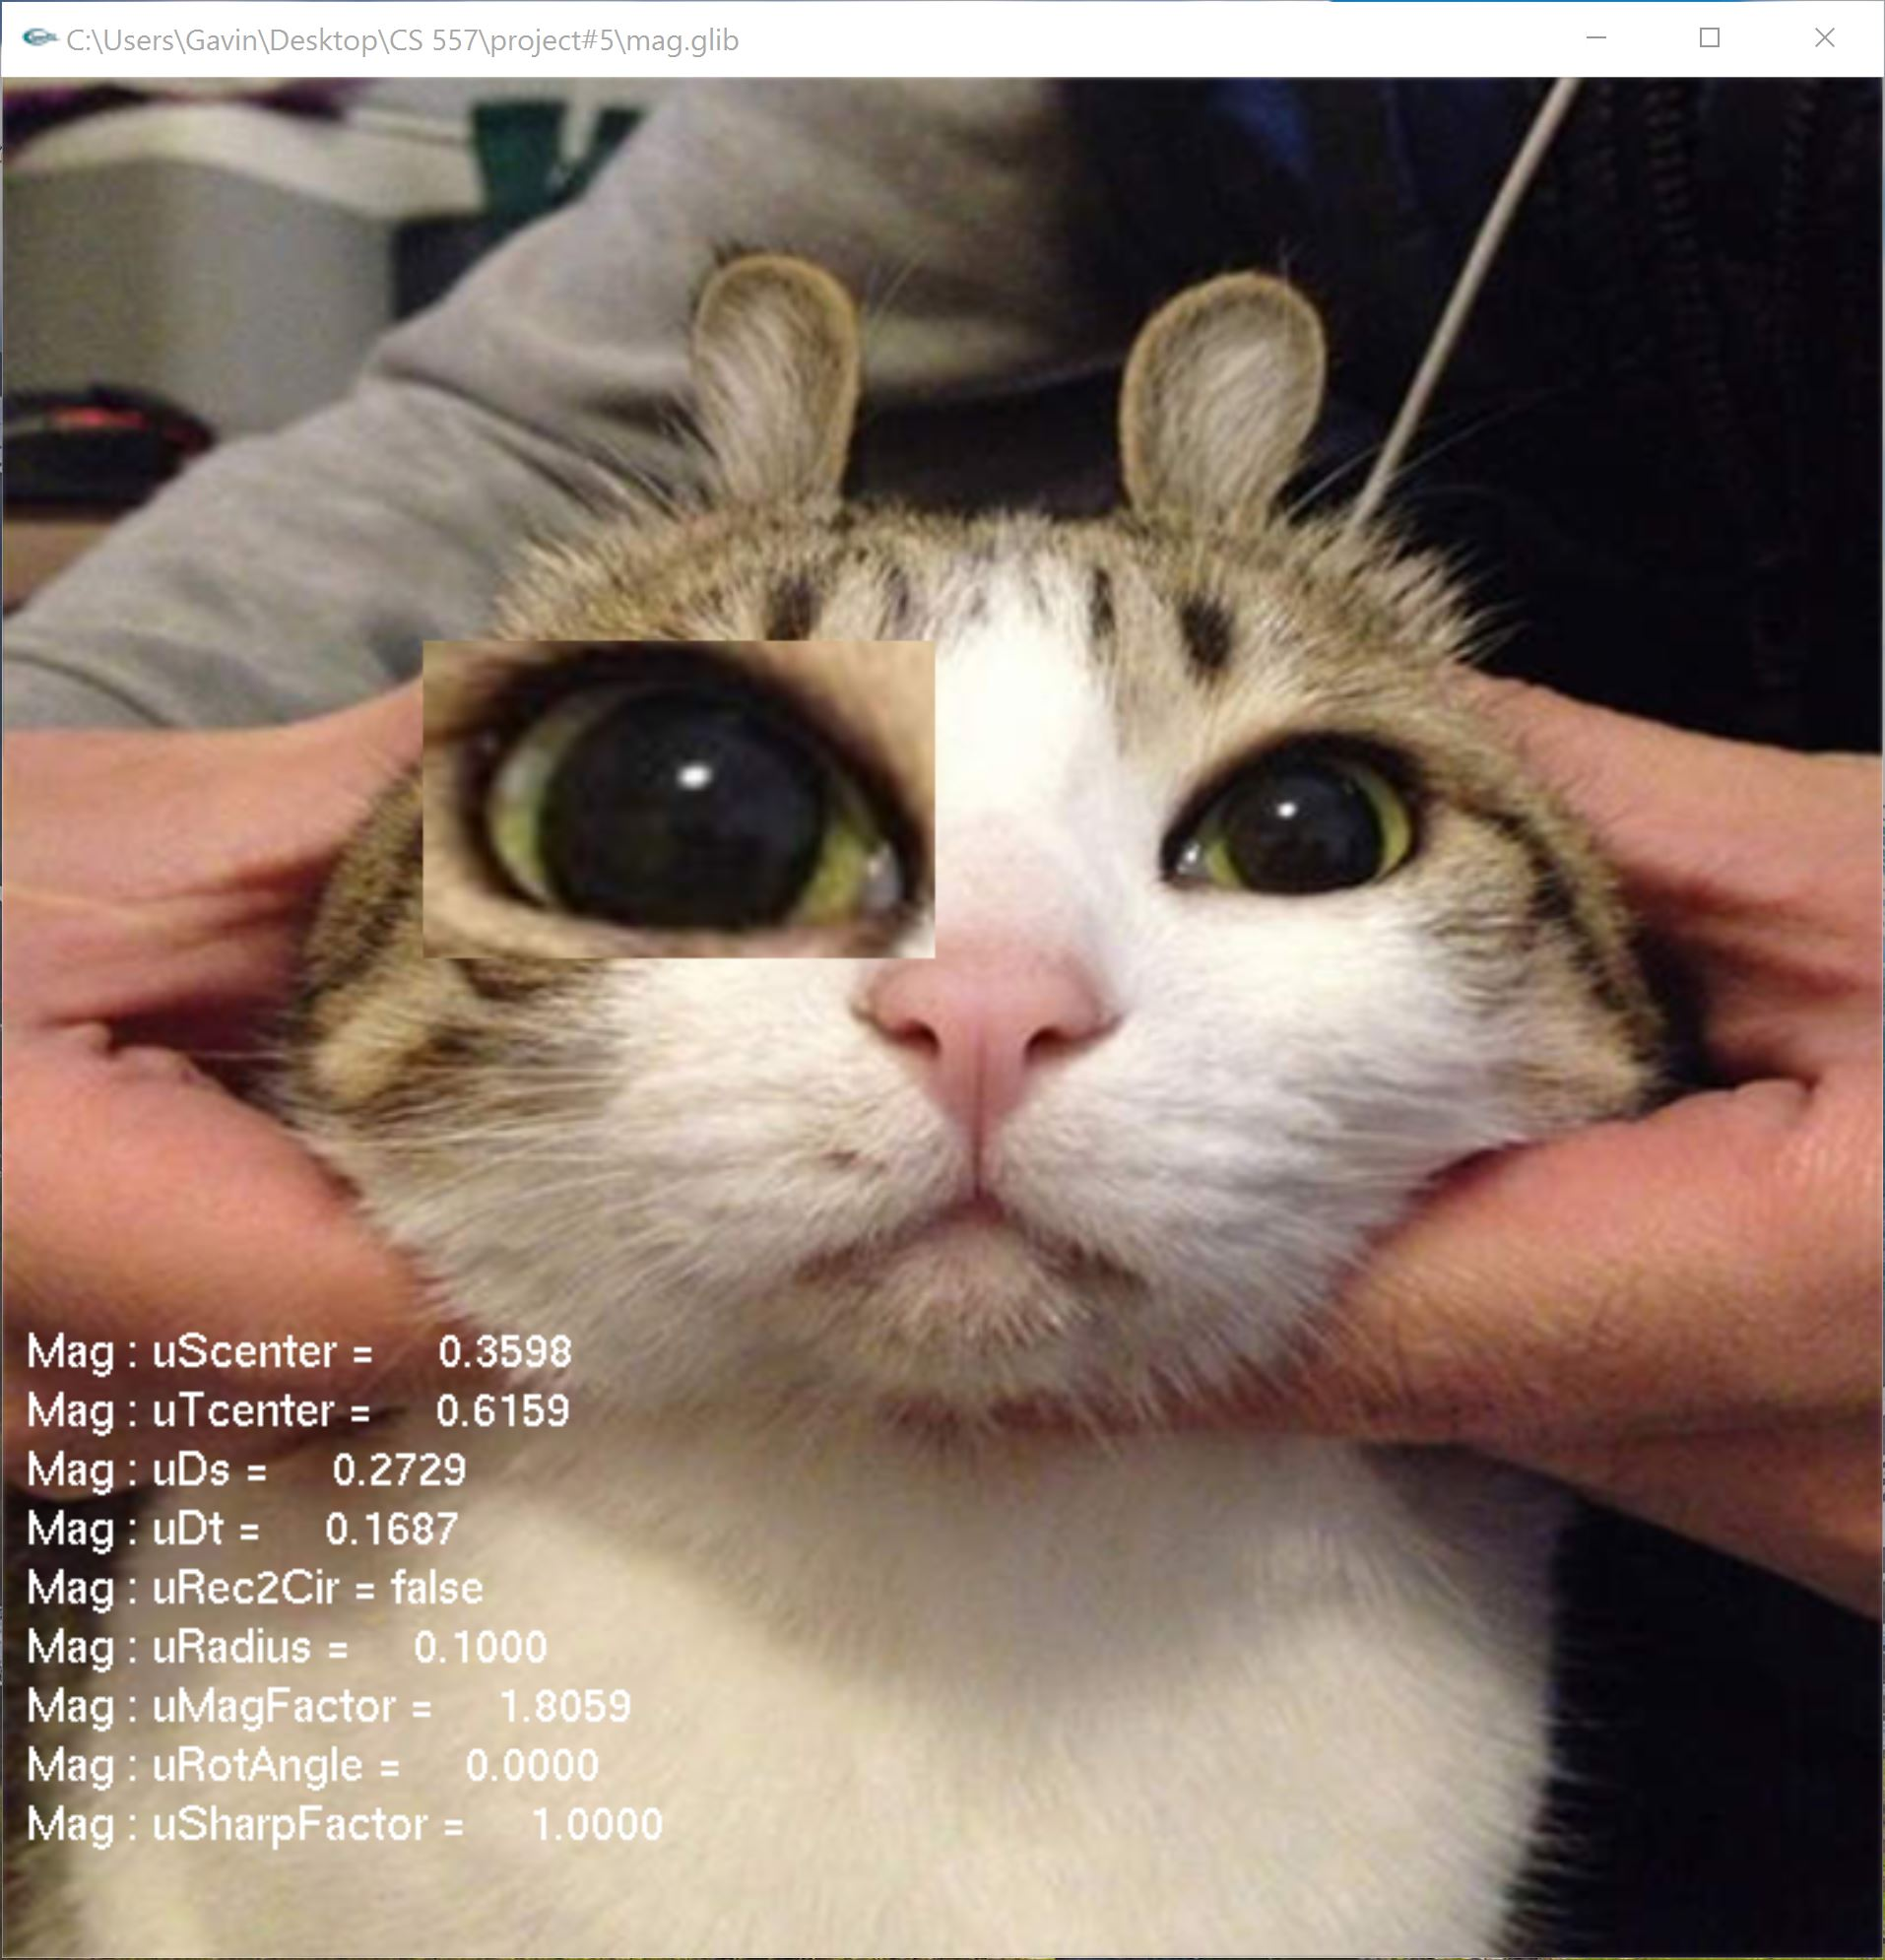
\includegraphics[width=3.2in]{mag.jpg}
	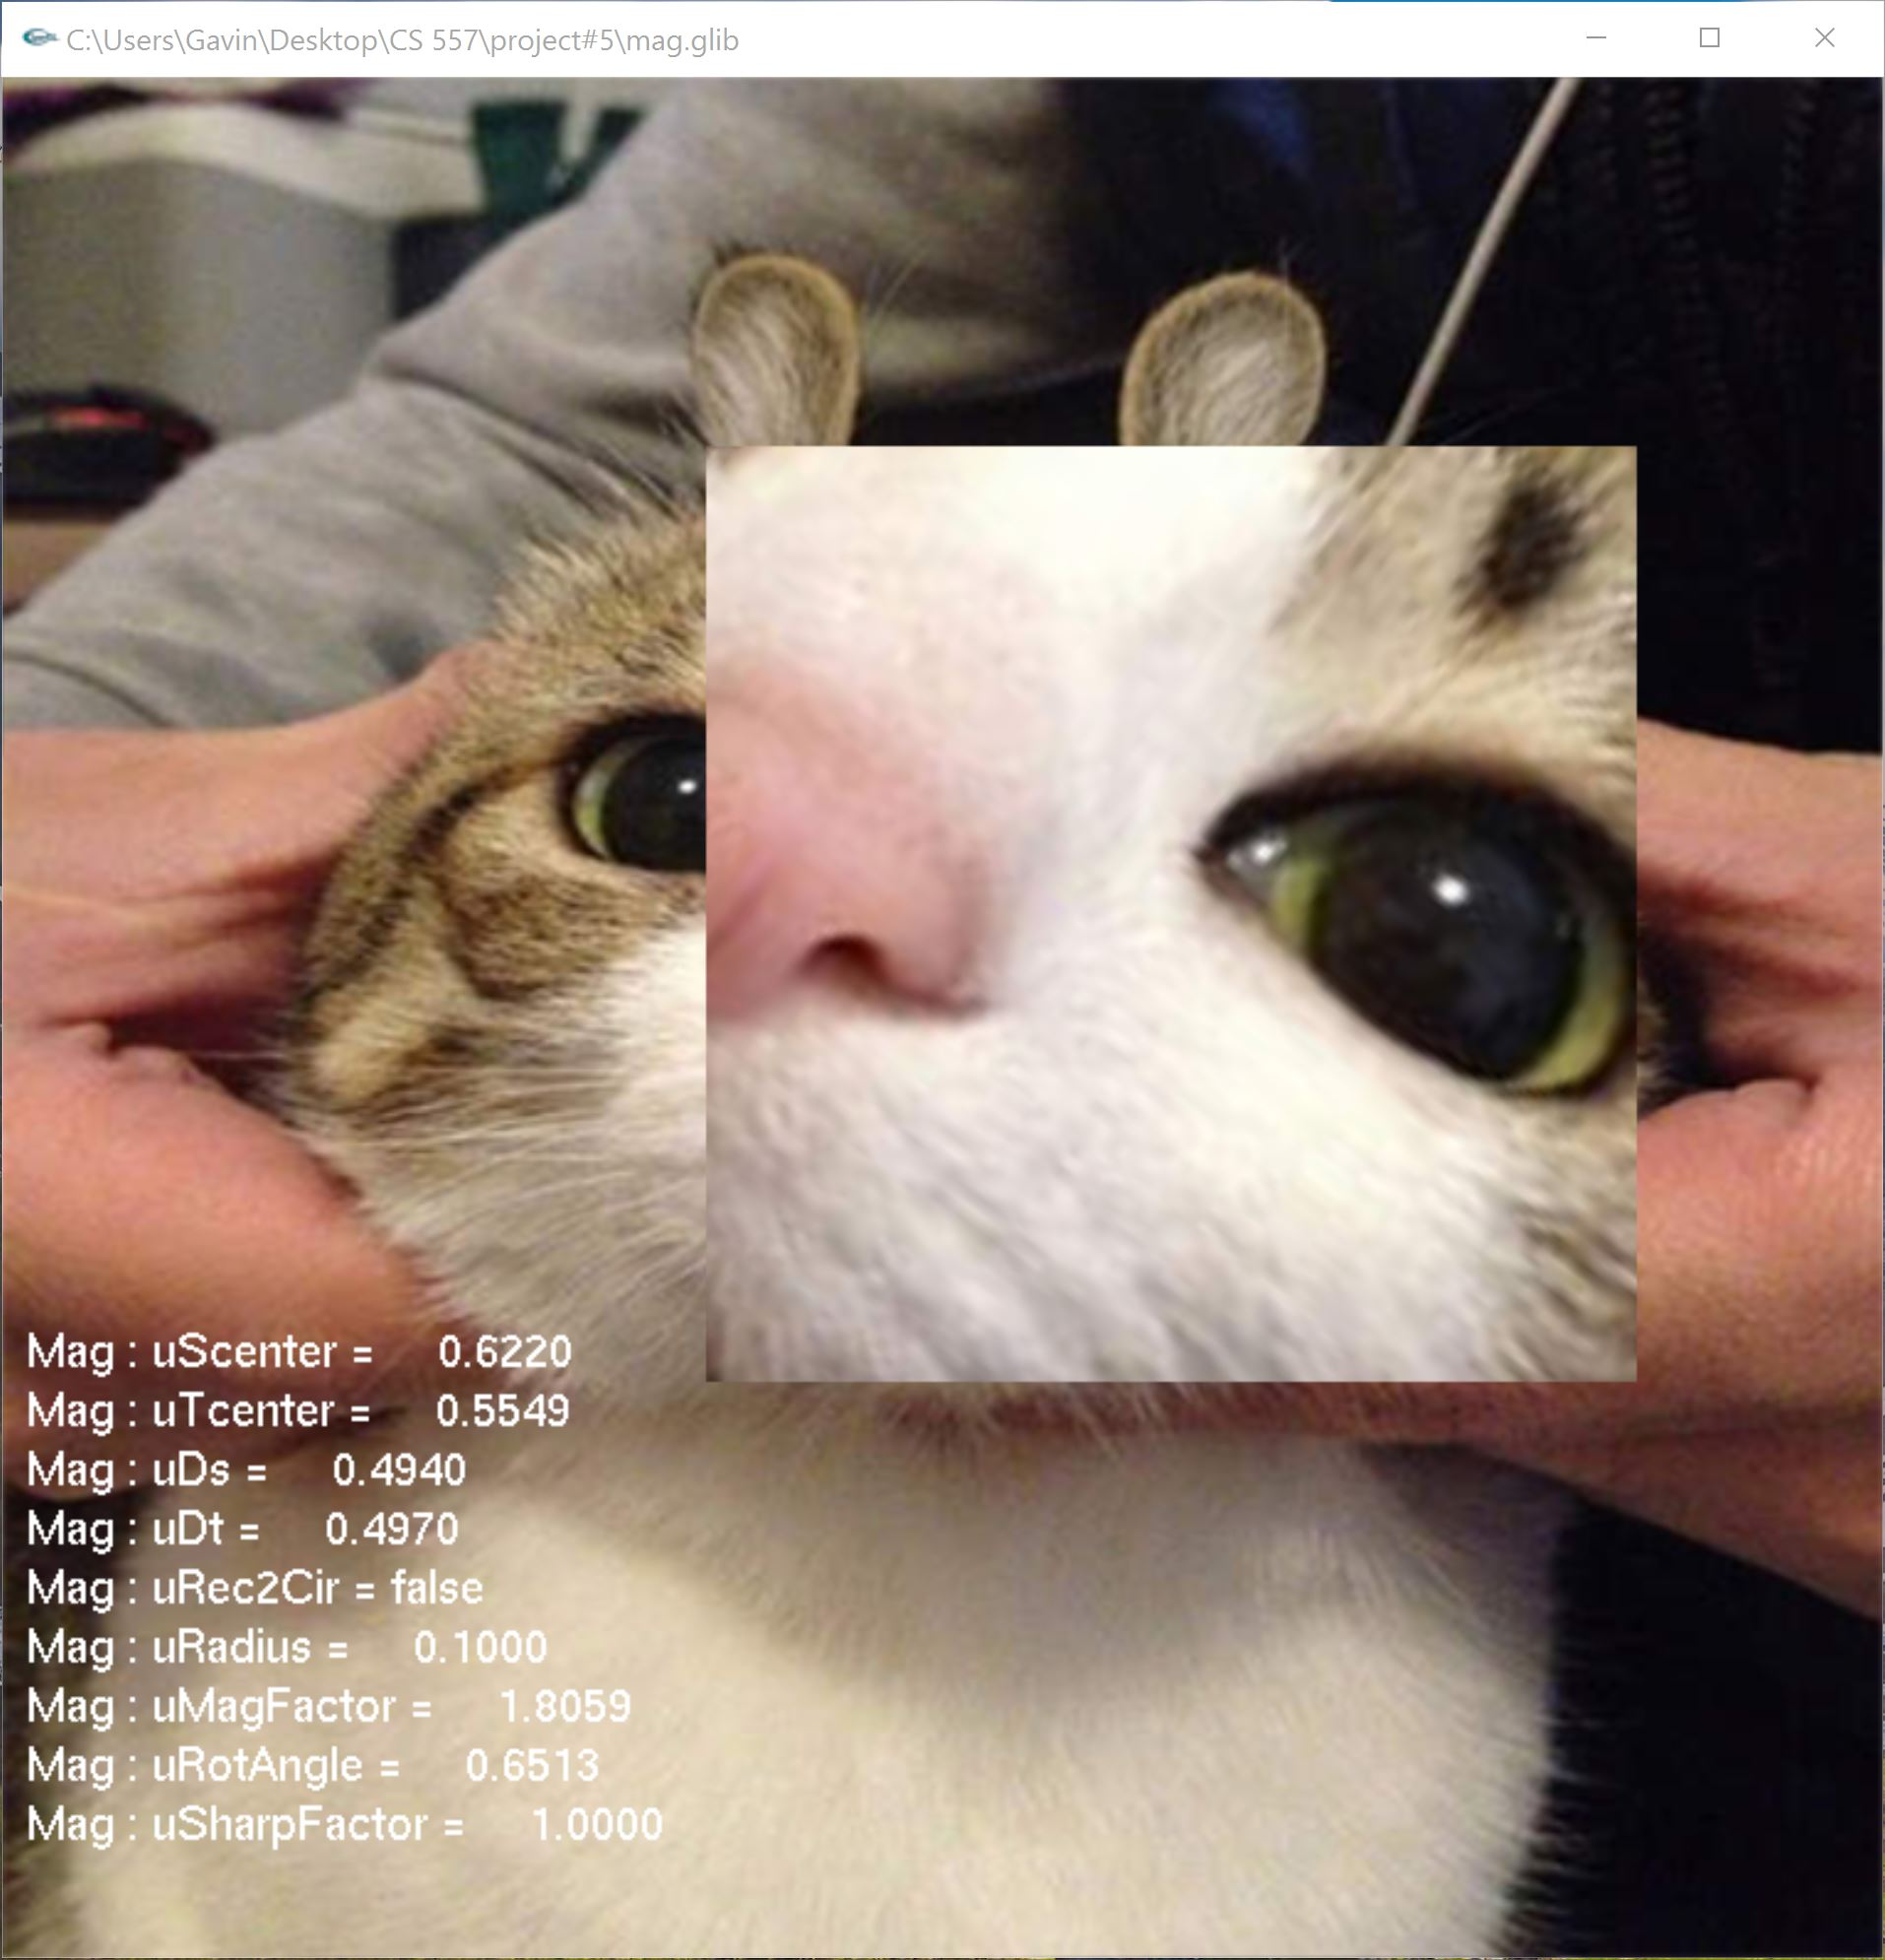
\includegraphics[width=3.2in]{rotate.jpg}
\end{center}
The second part of the project if rotation. The image covered by the lens will be rotate an angle from the slider ``uRotAngle''. As it mentioned in the project website, to rotate the image we need to apply the equations $x' = x*cos(theta) - y*sin(theta)$ and $y' = x*sin(theta) + y*cos(theta)$. However for this assignment, we need to manipulate the st coordinates instead of the xt coordinates, and the rotate center should be the center of the lens, so I created the following equations instead: $sp = uScenter+((stp.s-uScenter)*cos(uRotAngle)-(stp.t-uTcenter)*sin(uRotAngle))$ and $tp = uTcenter+((stp.s-uScenter)*sin(uRotAngle)+(stp.t-uTcenter)*cos(uRotAngle))$. The rotation effect is shown in the above right image.

The third part of this project is the sharpening. To implement the sharpening we simply apply the blur matrix to the image. the blur matrix simply blur the part that we don't need in the image in order to deliver the sharpening effects. The example code has already been given in the class notes, and the changes that need to be applied to it are just changing the original st coordinates to the current coordinates that have been enlarged and rotated. The following image shows the effect of sharpening. The details on the fur of the cat delivered a clear idea of how the sharpening works.
\begin{center}
	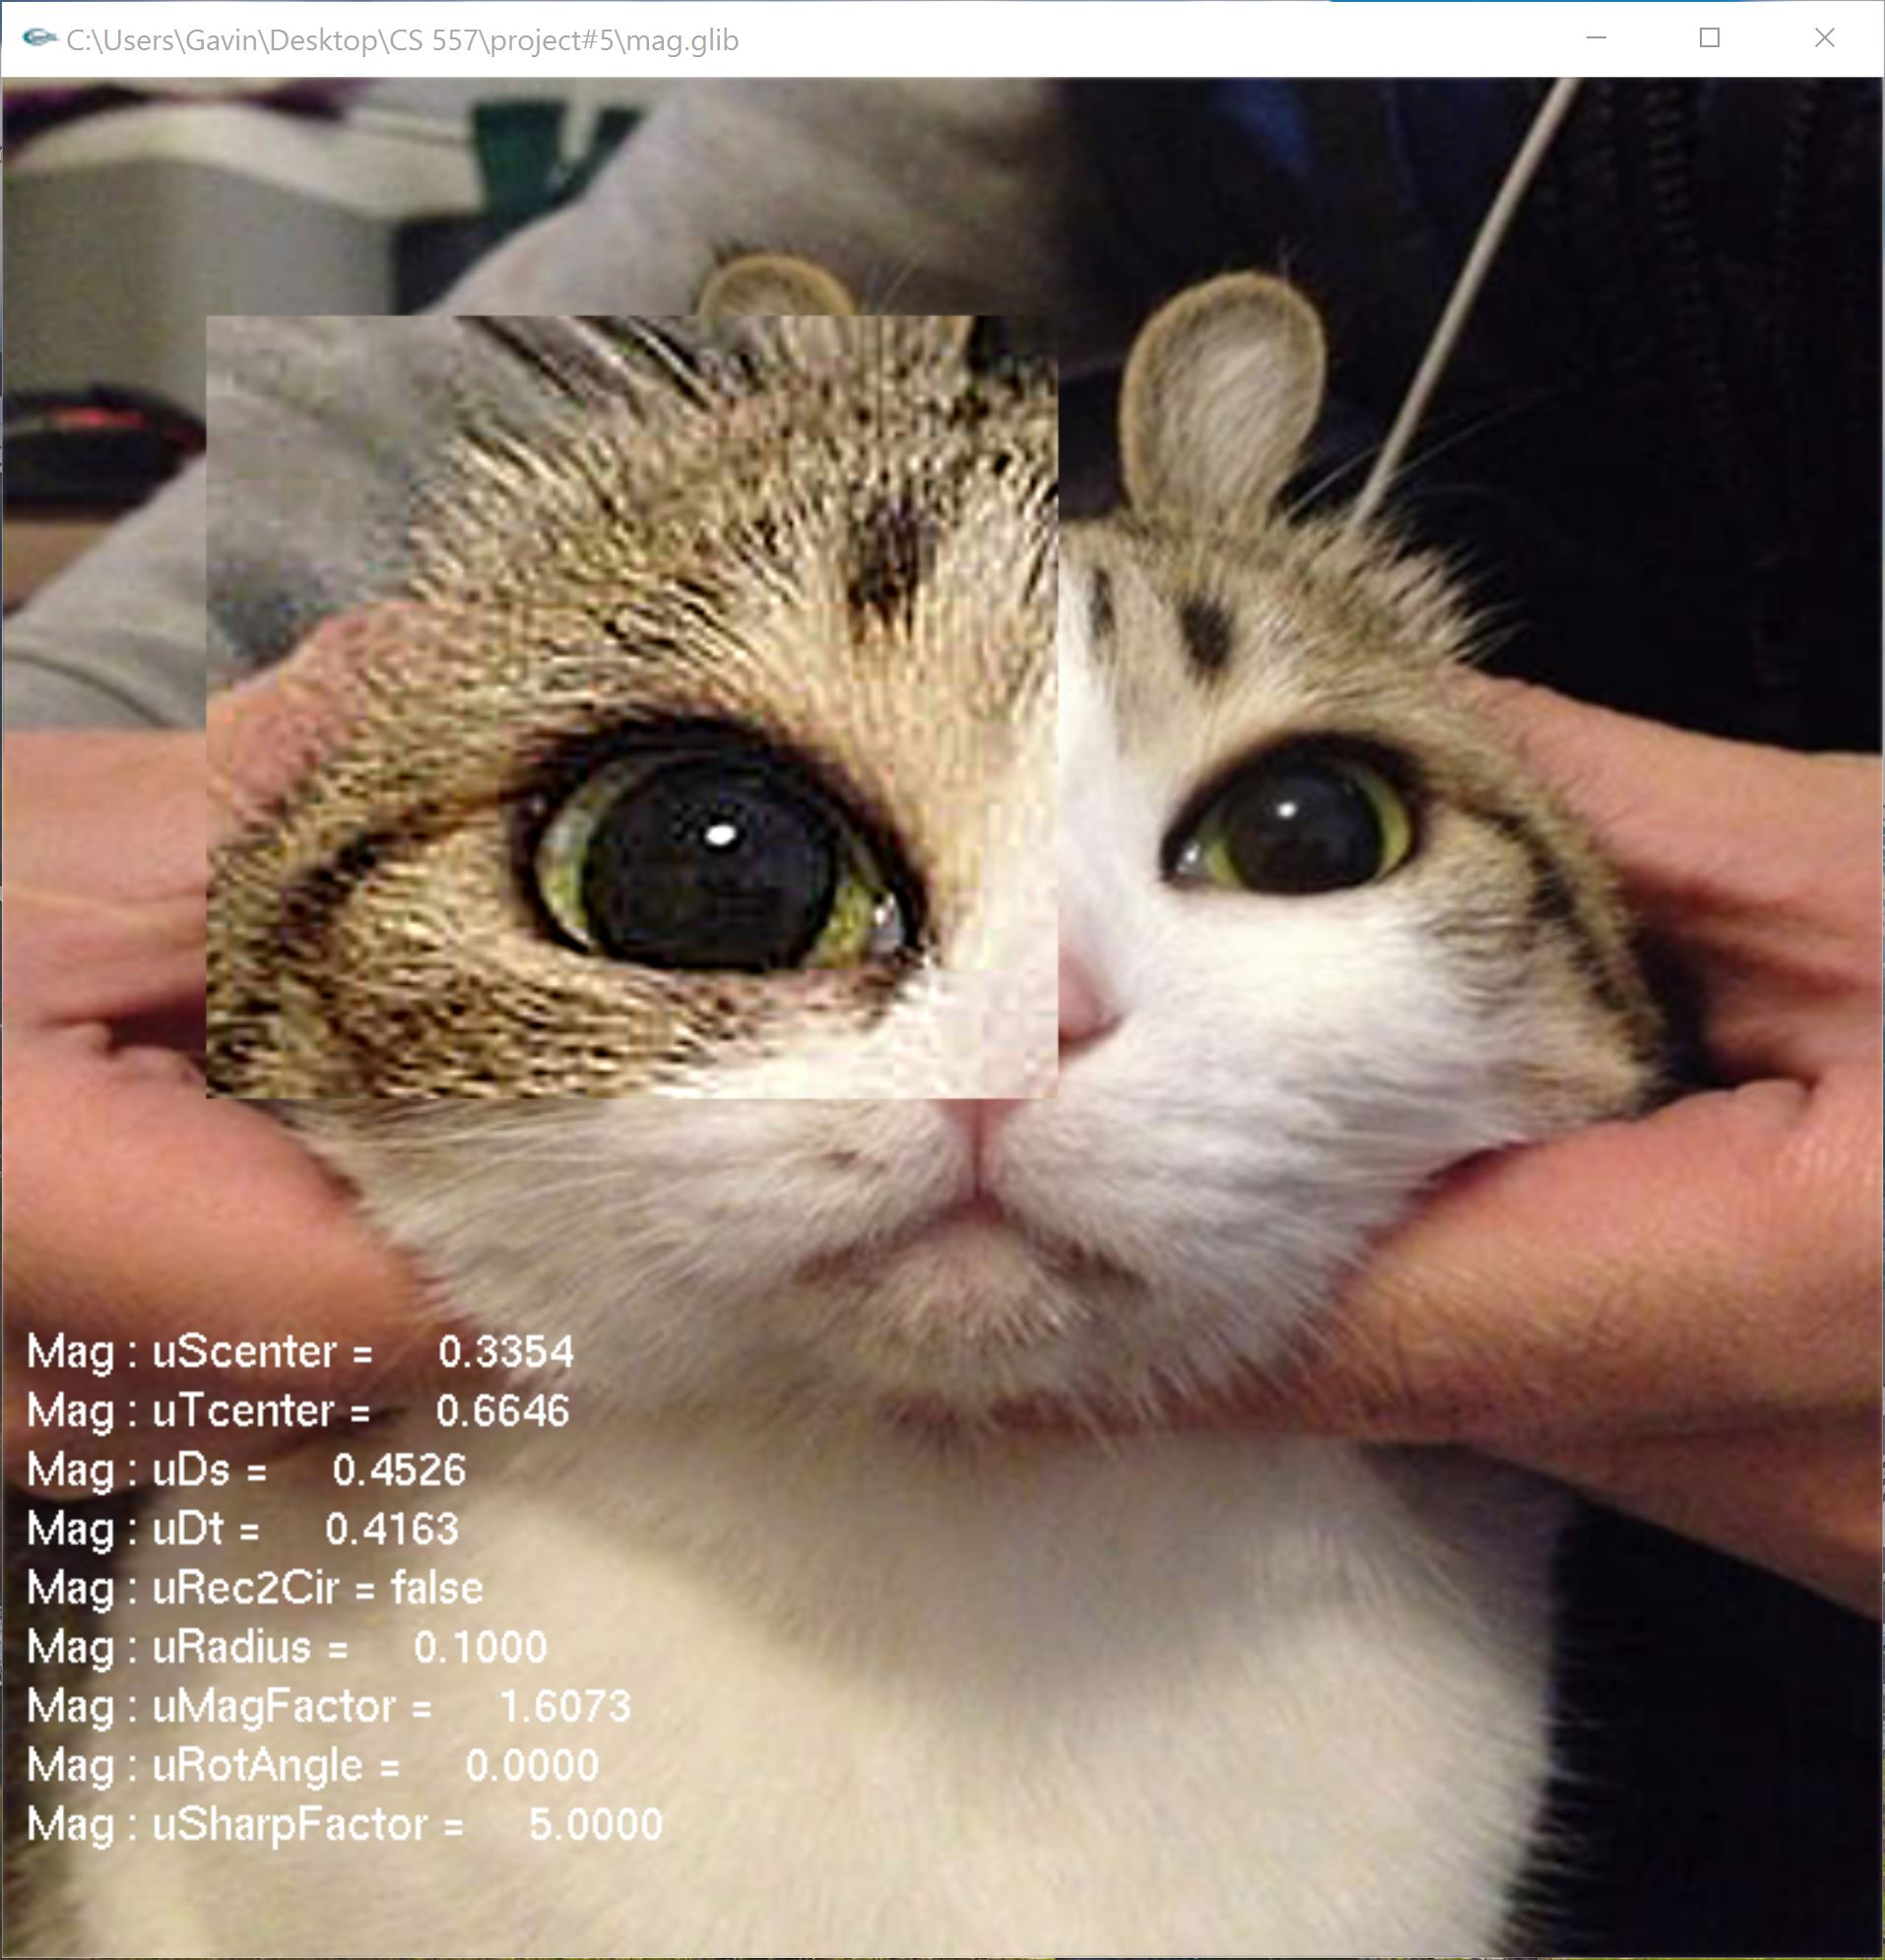
\includegraphics[width=3.2in]{sharpen.jpg}
\end{center}
The final part of the project is the extra credit part. It requires changing the lens from rectangle to circle. Basically, what we have done for scaling, rotation and sharpening stays the same, and the only thing that needs to be changed is the way we determine whether the texel is in the lens or not. Instead of checking the boundary of the rectangle, I simply calculate the distance from the selected texel to the lens center. If the distance is smaller than the radius of the circle, then it is in the lens, otherwise it's not. The effects of circle lens with scaling, rotation and sharpening is shown in the following image.
\begin{center}
	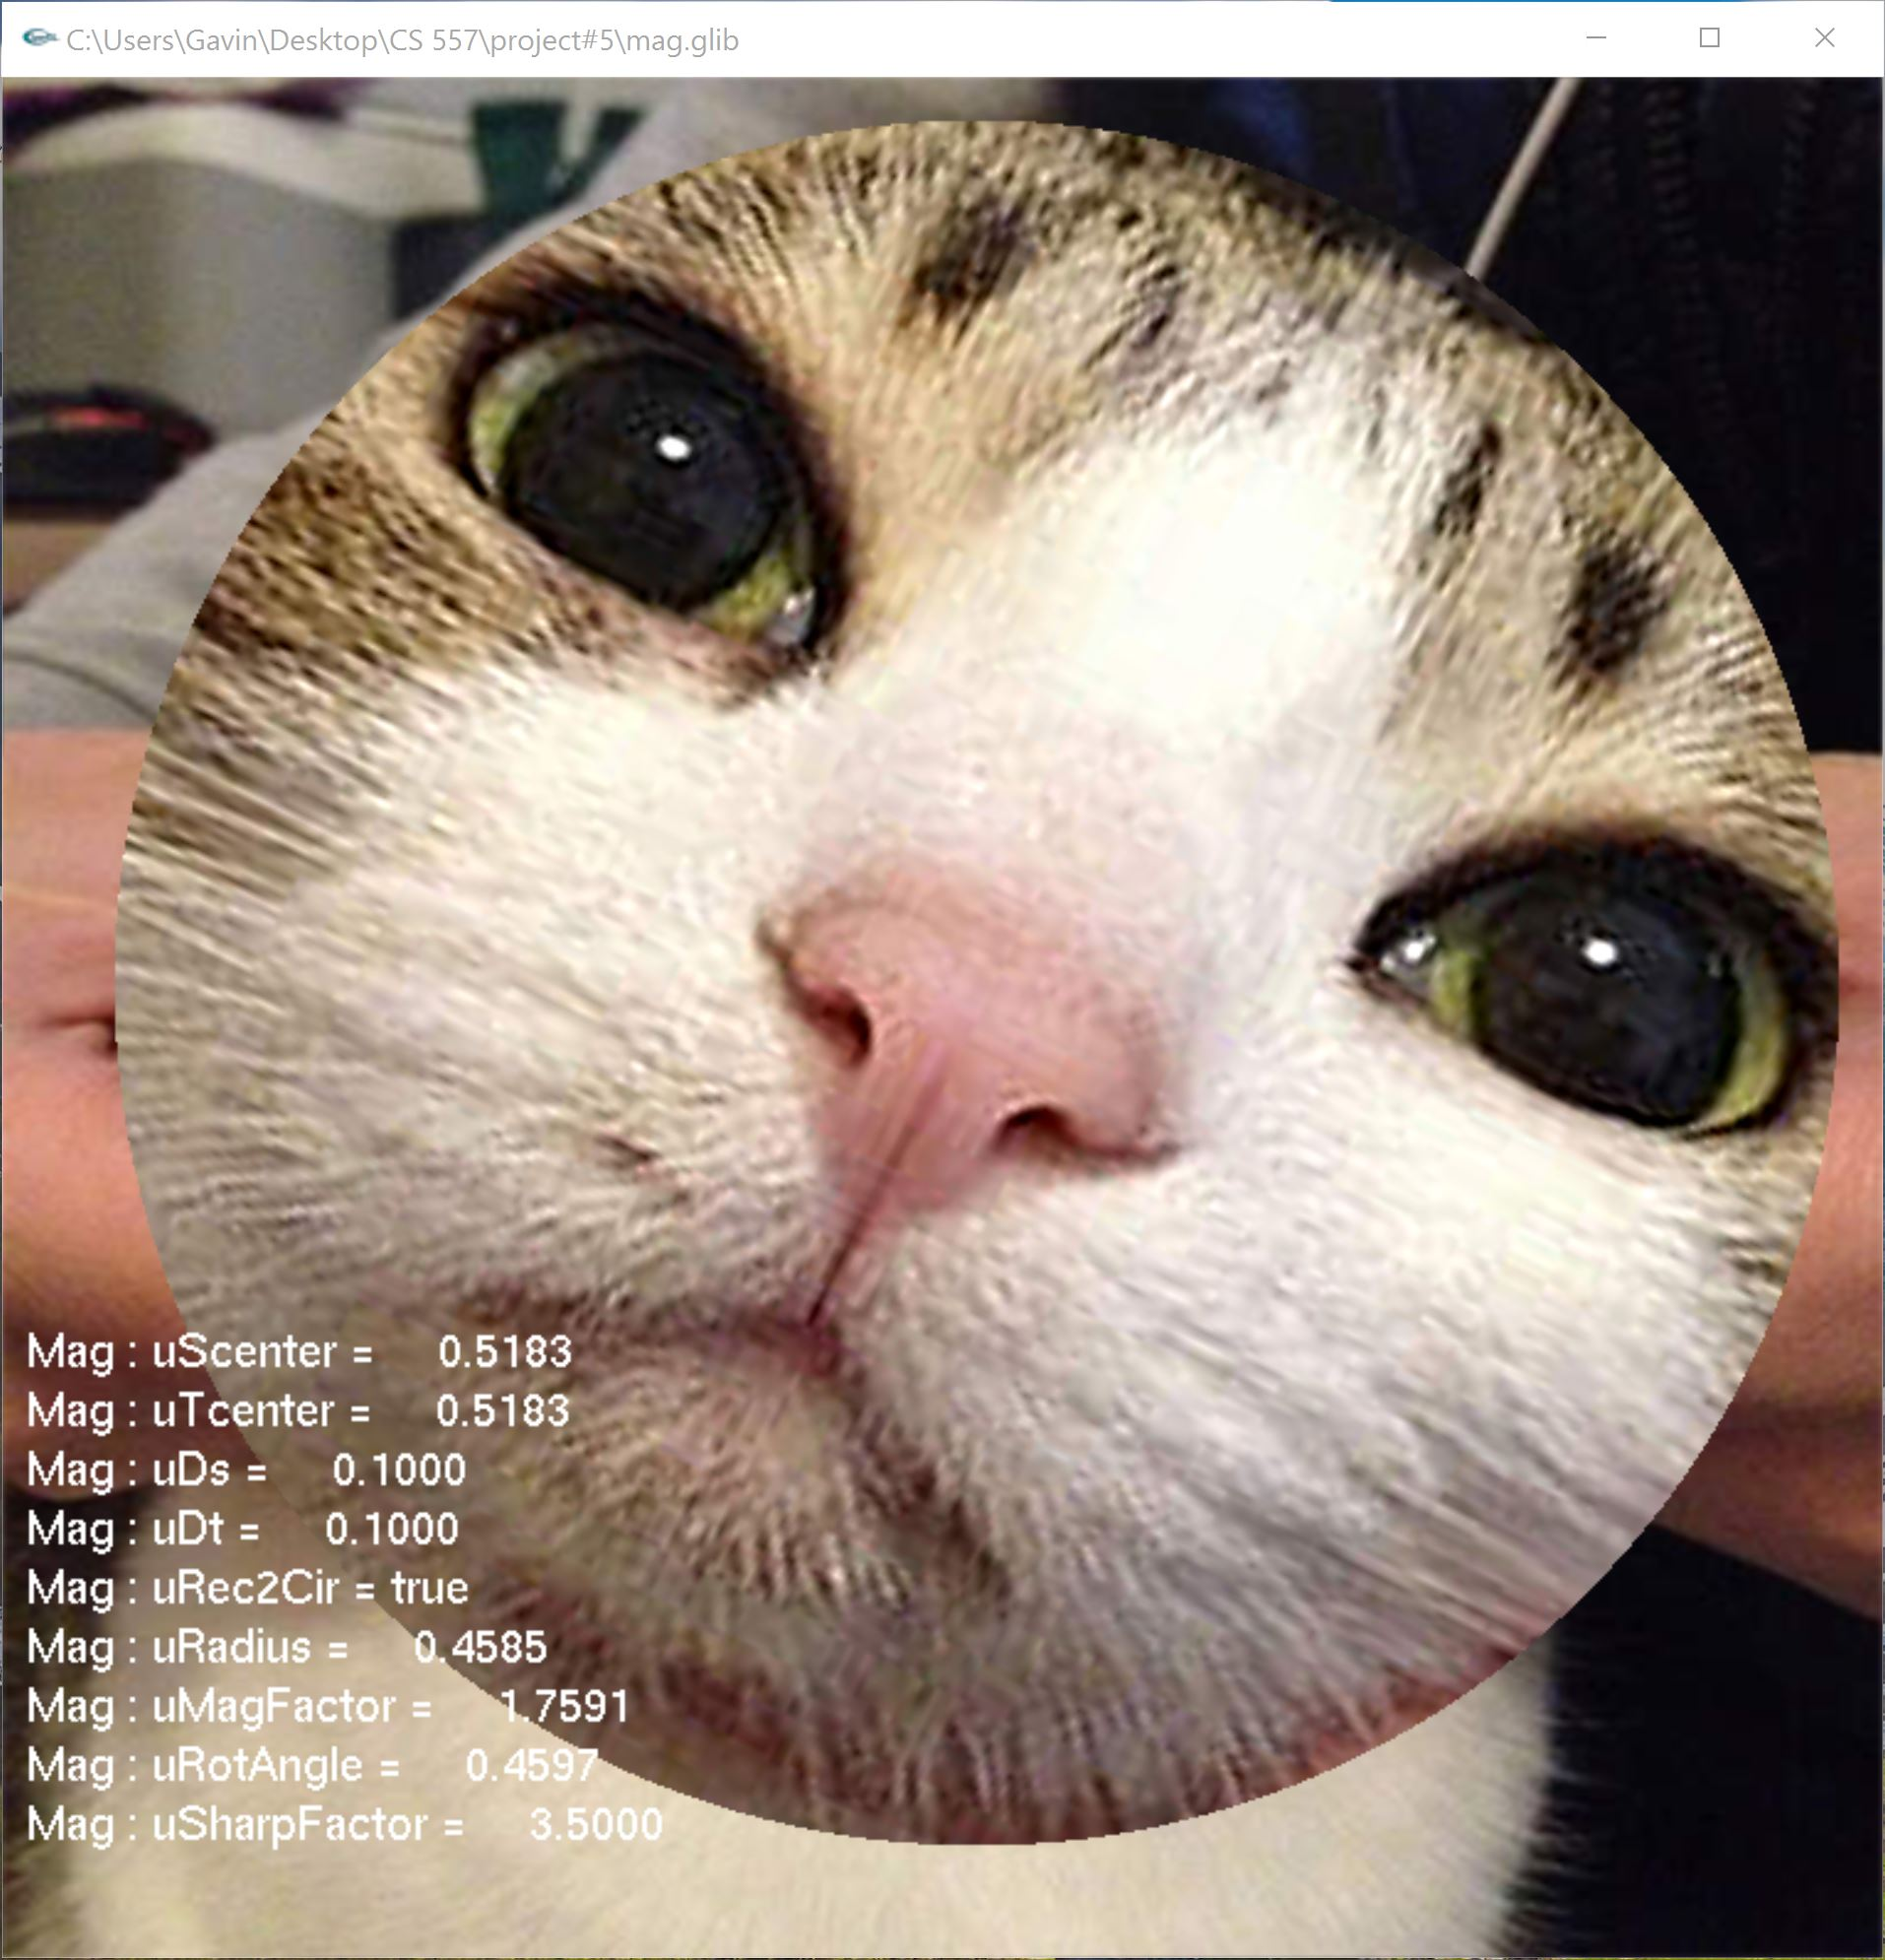
\includegraphics[width=3.75in]{circle.jpg}
\end{center}
\section{Summary}
This project is pretty easy to handle, and the effects is really fun to play with. Manipulating the st coordinates gives me a deeper understanding of the texture. I'm looking forward to other projects in this class and eager to do them well.
\end{document}